
%(BEGIN_QUESTION)
% Copyright 2006, Tony R. Kuphaldt, released under the Creative Commons Attribution License (v 1.0)
% This means you may do almost anything with this work of mine, so long as you give me proper credit

Determine the final effect of each fault for this pneumatic force-balance system:

$$\includegraphics[width=15.5cm]{i00202x01.eps}$$

\begin{itemize}
\item{} Clogged nozzle
\item{} Clogged restriction
\item{} Clogged tube at supply port of amplifying relay
\item{} Broken leaf spring inside amplifying relay
\item{} Major hole or tear in diaphragm inside amplifying relay
\end{itemize}

Be sure to explain the final effects for each of these faults!

\underbar{file i00202}
%(END_QUESTION)





%(BEGIN_ANSWER)

\begin{itemize}
\item{} Clogged nozzle: {\it output pressure saturates high}
\item{} Clogged restriction: {\it output pressure saturates low}
\item{} Clogged tube at supply port of amplifying relay: {\it output pressure saturates low}
\item{} Broken leaf spring inside amplifying relay: {\it output pressure may saturate high or possibly oscillate}
\item{} Major hole or tear in diaphragm inside amplifying relay: {\it System responds very little to applied force}
\end{itemize}

%(END_ANSWER)





%(BEGIN_NOTES)

The particular pneumatic amplifying relay shown is the one typically used in Foxboro pneumatic instruments.  It is not the only type of amplifying relay design, but a very common one.

%INDEX% Basics, pneumatics: force-balance mechanism

%(END_NOTES)


